
%-----------------------------------------
\section{Limits from inclusive event category without \text{c} tagging}
\label{ss:limit_Inc}
%-----------------------------------------
To extract possible signal, the $\mjj$ distribution as shown in Figures~\ref{subfig:mjj_kfit_muKinFit},~\ref{subfig:mjj_kfit_eleKinFit},~\ref{subfig:mjj_sig_kfit_mu}, and \ref{subfig:mjj_sig_kfit_ele} are used in a binned maximum-likelihood fit. The upper limit on the \brThb as a function of $m_{H^{+}}$ is 
shown in Figures~\ref{subfig:limit_mu_Inc},~\ref{subfig:limit_ele_Inc}, and \ref{subfig:limit_lep_Inc}
for the \mujets and \ejets and \ljets channel, respectively. 
Corresponding values of the expected (observed) limits, for the charged Higgs mass 
from 90 to 160 \GeV, are in the range 0.40--1.42\% (0.32--0.98\%), 0.44--1.57\% (0.28--2.35\%), 
and 0.32--1.08\% (0.18--1.04) respectively. The expected (observed) limits using $\mjj$ from 
inclusive event category at 8 \TeV was in range 1.4--3.6\% (1.2--6.5\%) for \ljets 
channel~\cite{Khachatryan:2015uua}.
\begin{figure}
    \centering  
    \subfigure[Without \PQc tagging \label{subfig:limit_mu_Inc}]
    {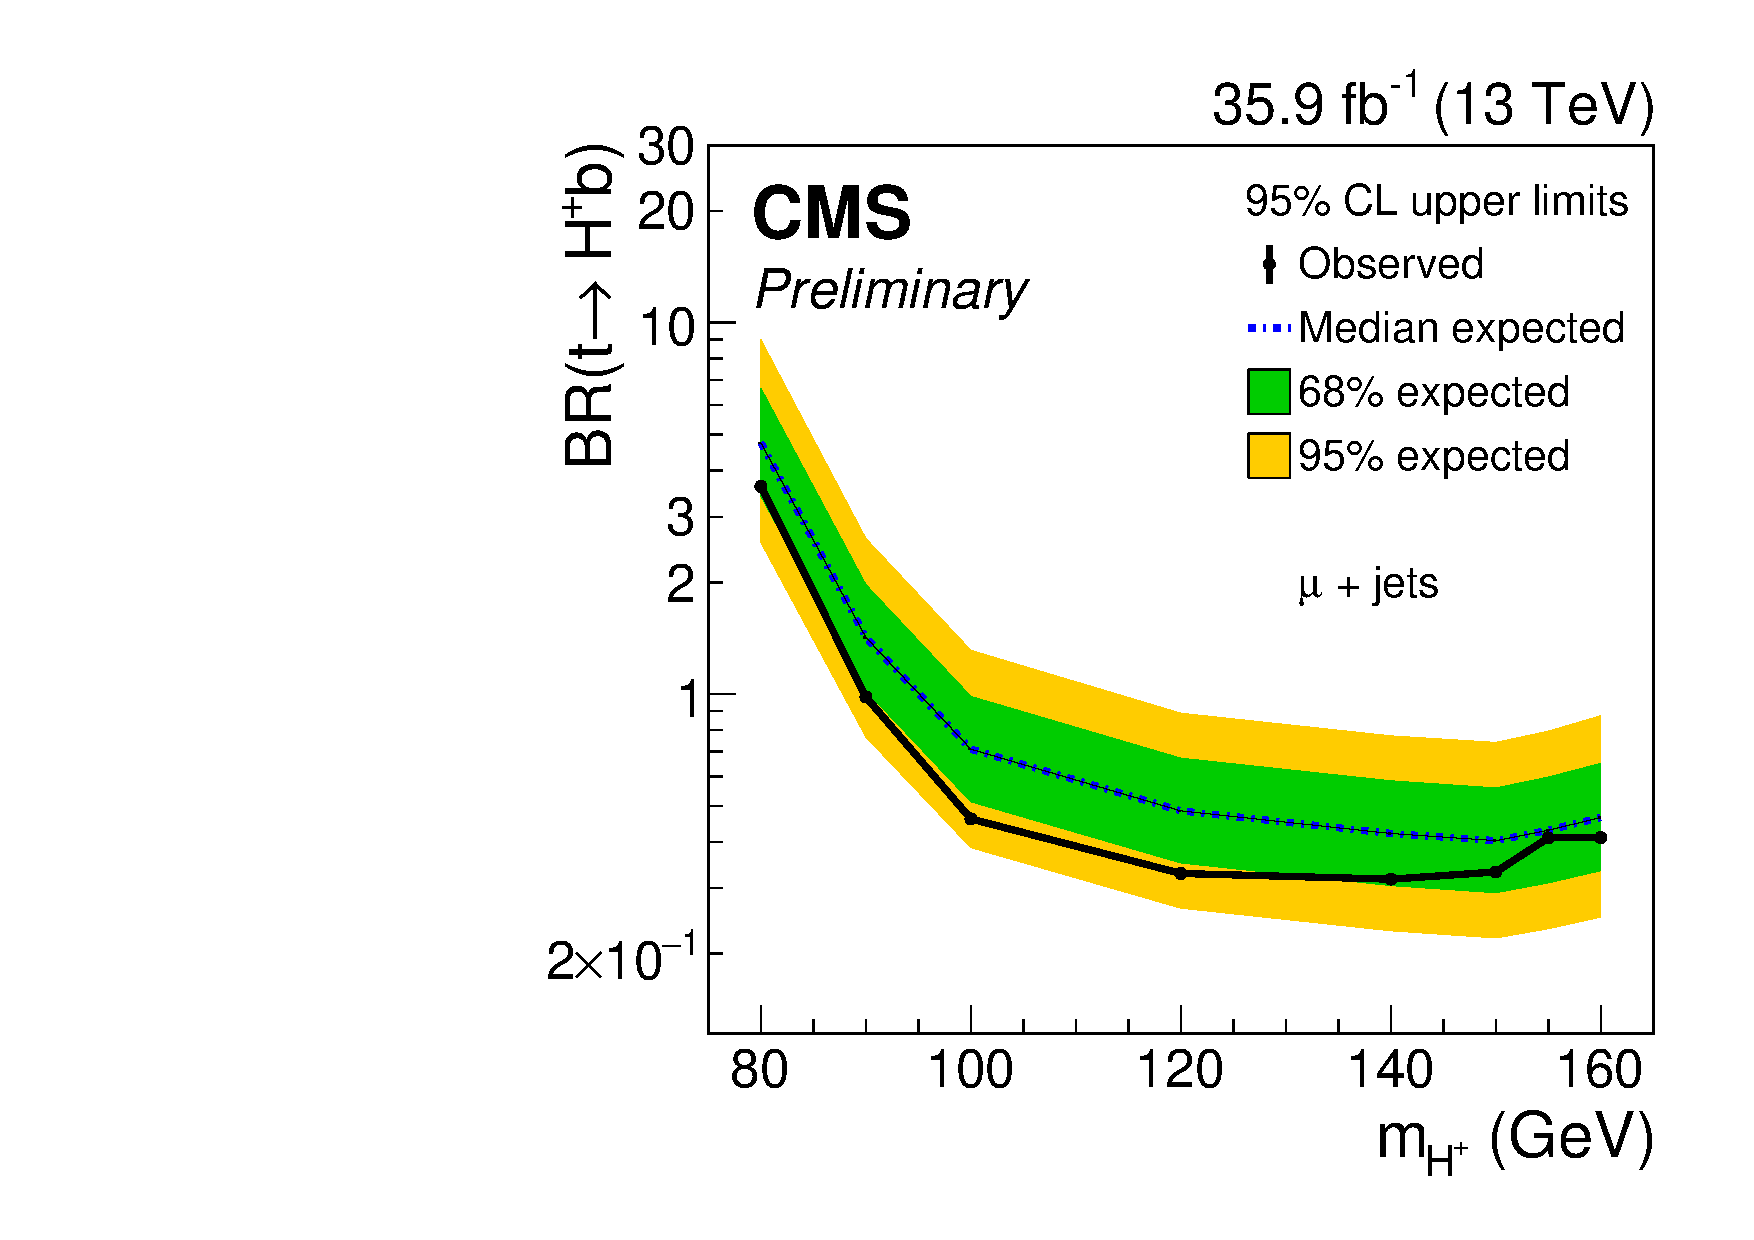
\includegraphics[width=0.30\linewidth]{Image/Limit/limit_pdf/limit_mu_Cat1_Inc.pdf}}
    \subfigure[Without \PQc tagging \label{subfig:limit_ele_Inc}]
    {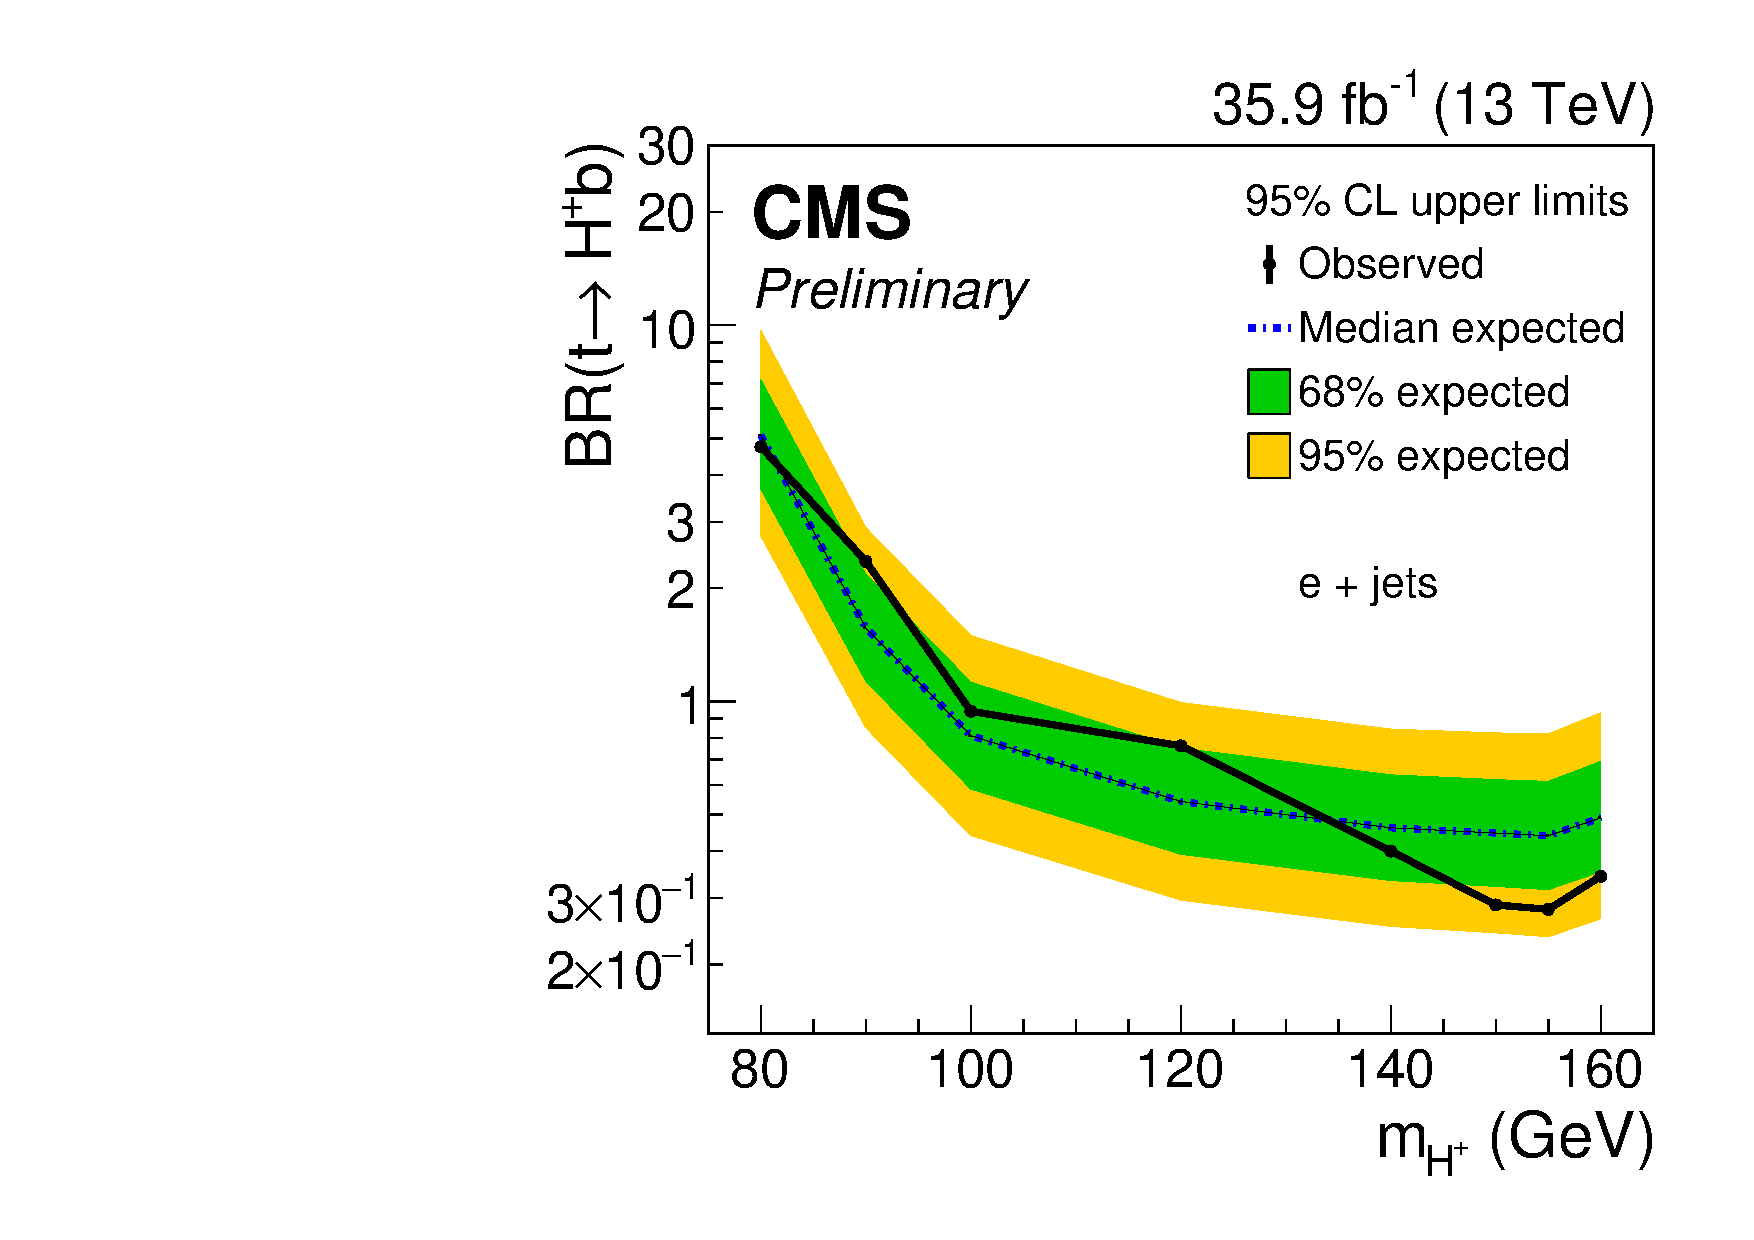
\includegraphics[width=0.30\linewidth]{Image/Limit/limit_pdf/limit_ele_Cat1_Inc.pdf}}
    \subfigure[Without \PQc tagging \label{subfig:limit_lep_Inc}]
    {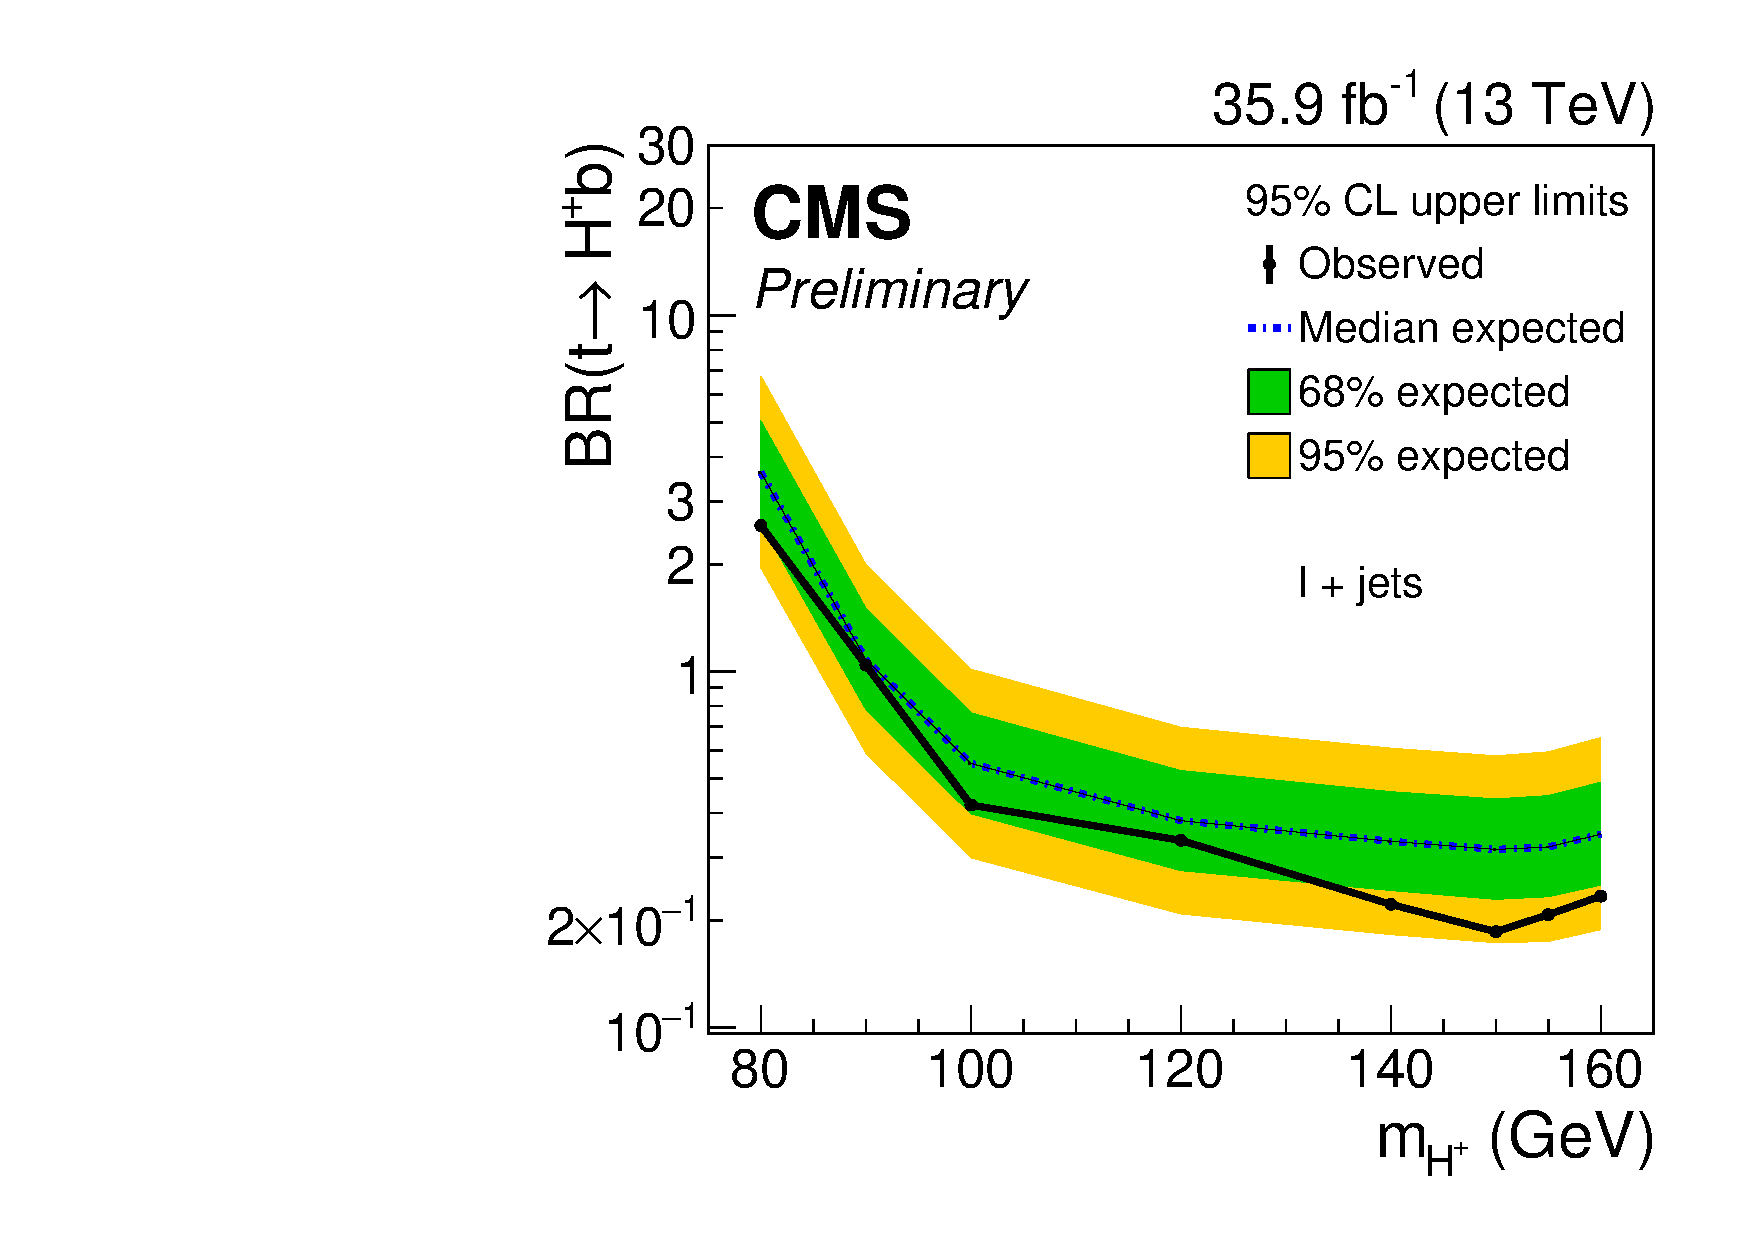
\includegraphics[width=0.30\linewidth]{Image/Limit/limit_pdf/limit_mu_ele_Cat1_Inc.pdf}}
    \vfil
    \subfigure[With loose \PQc tagging \label{subfig:limit_mu_cTagL}]
    {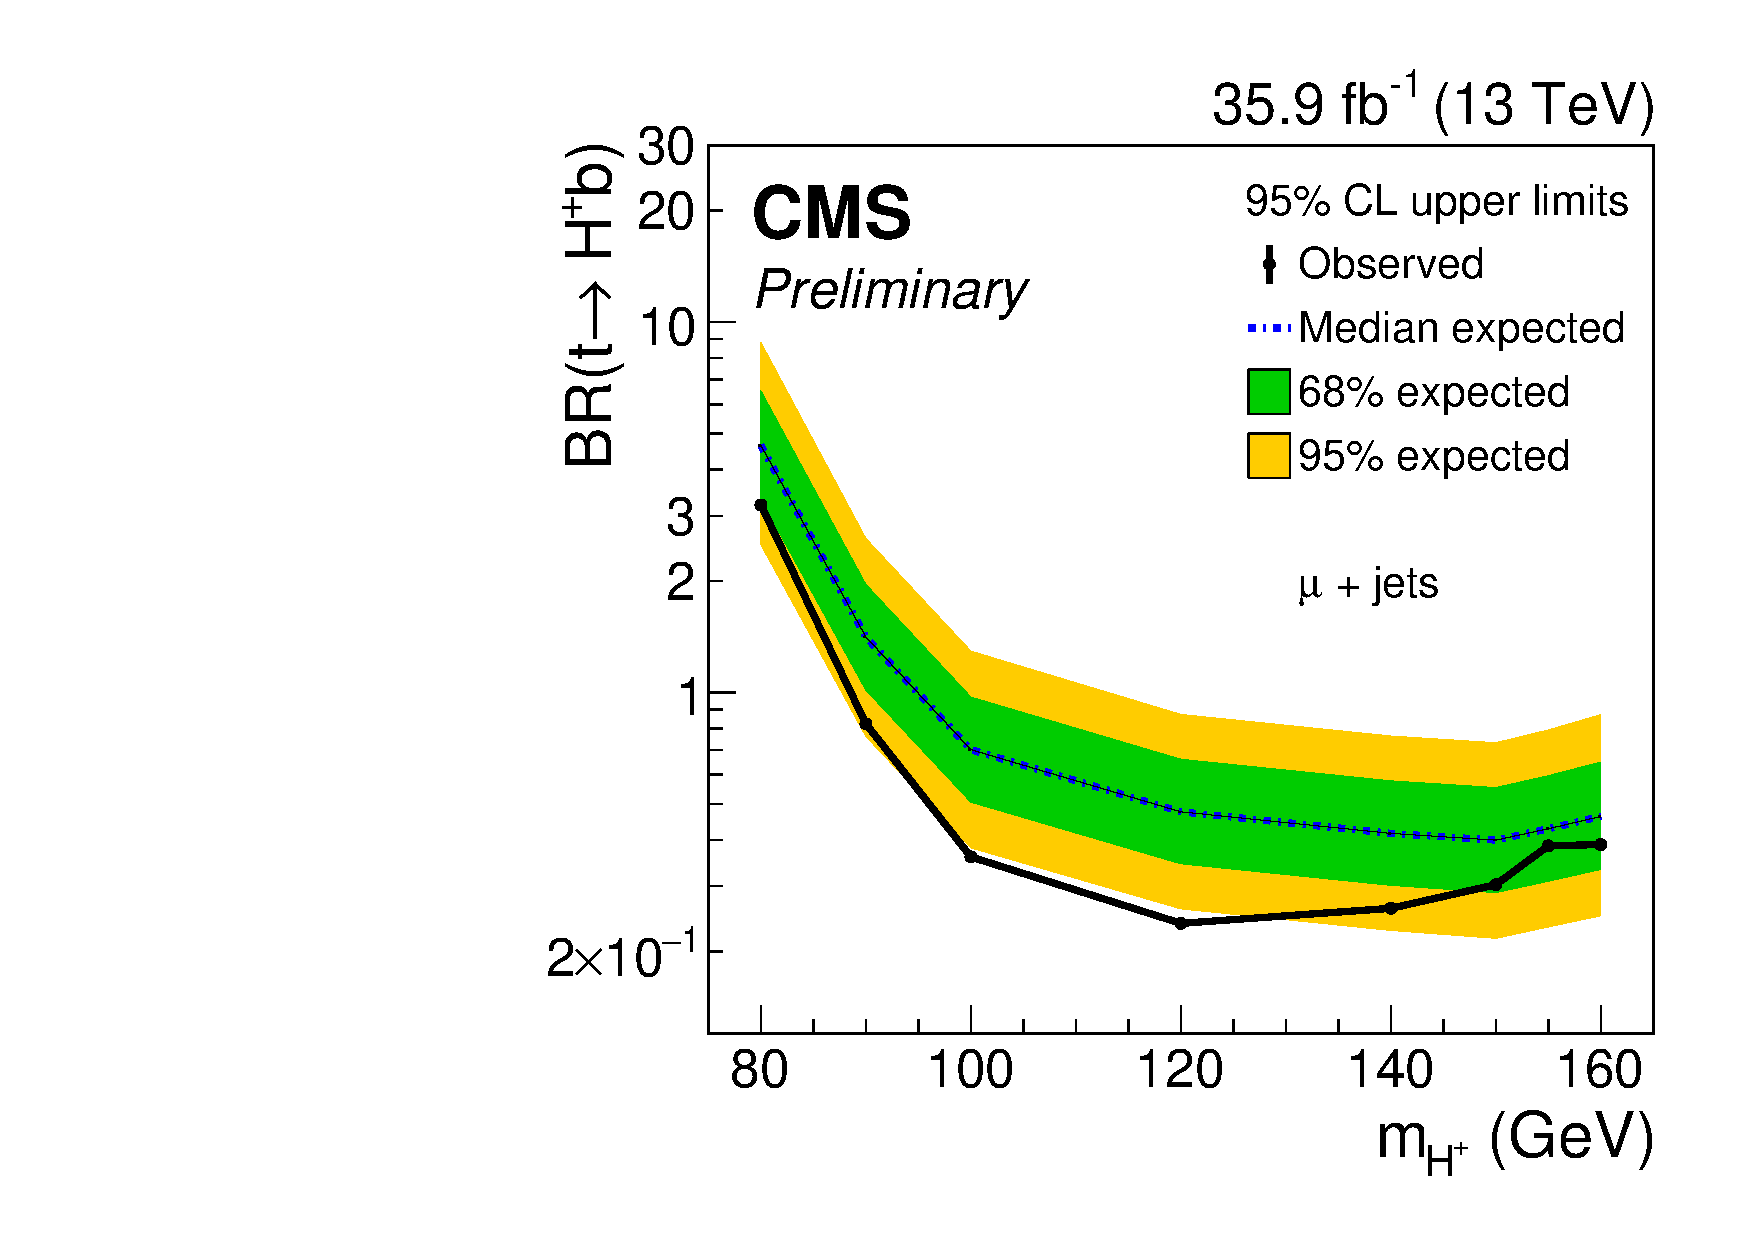
\includegraphics[width=0.30\linewidth]{Image/Limit/limit_pdf/limit_mu_Cat2_cTagInc.pdf}}
    \subfigure[With loose \PQc tagging \label{subfig:limit_ele_cTagL}]
    {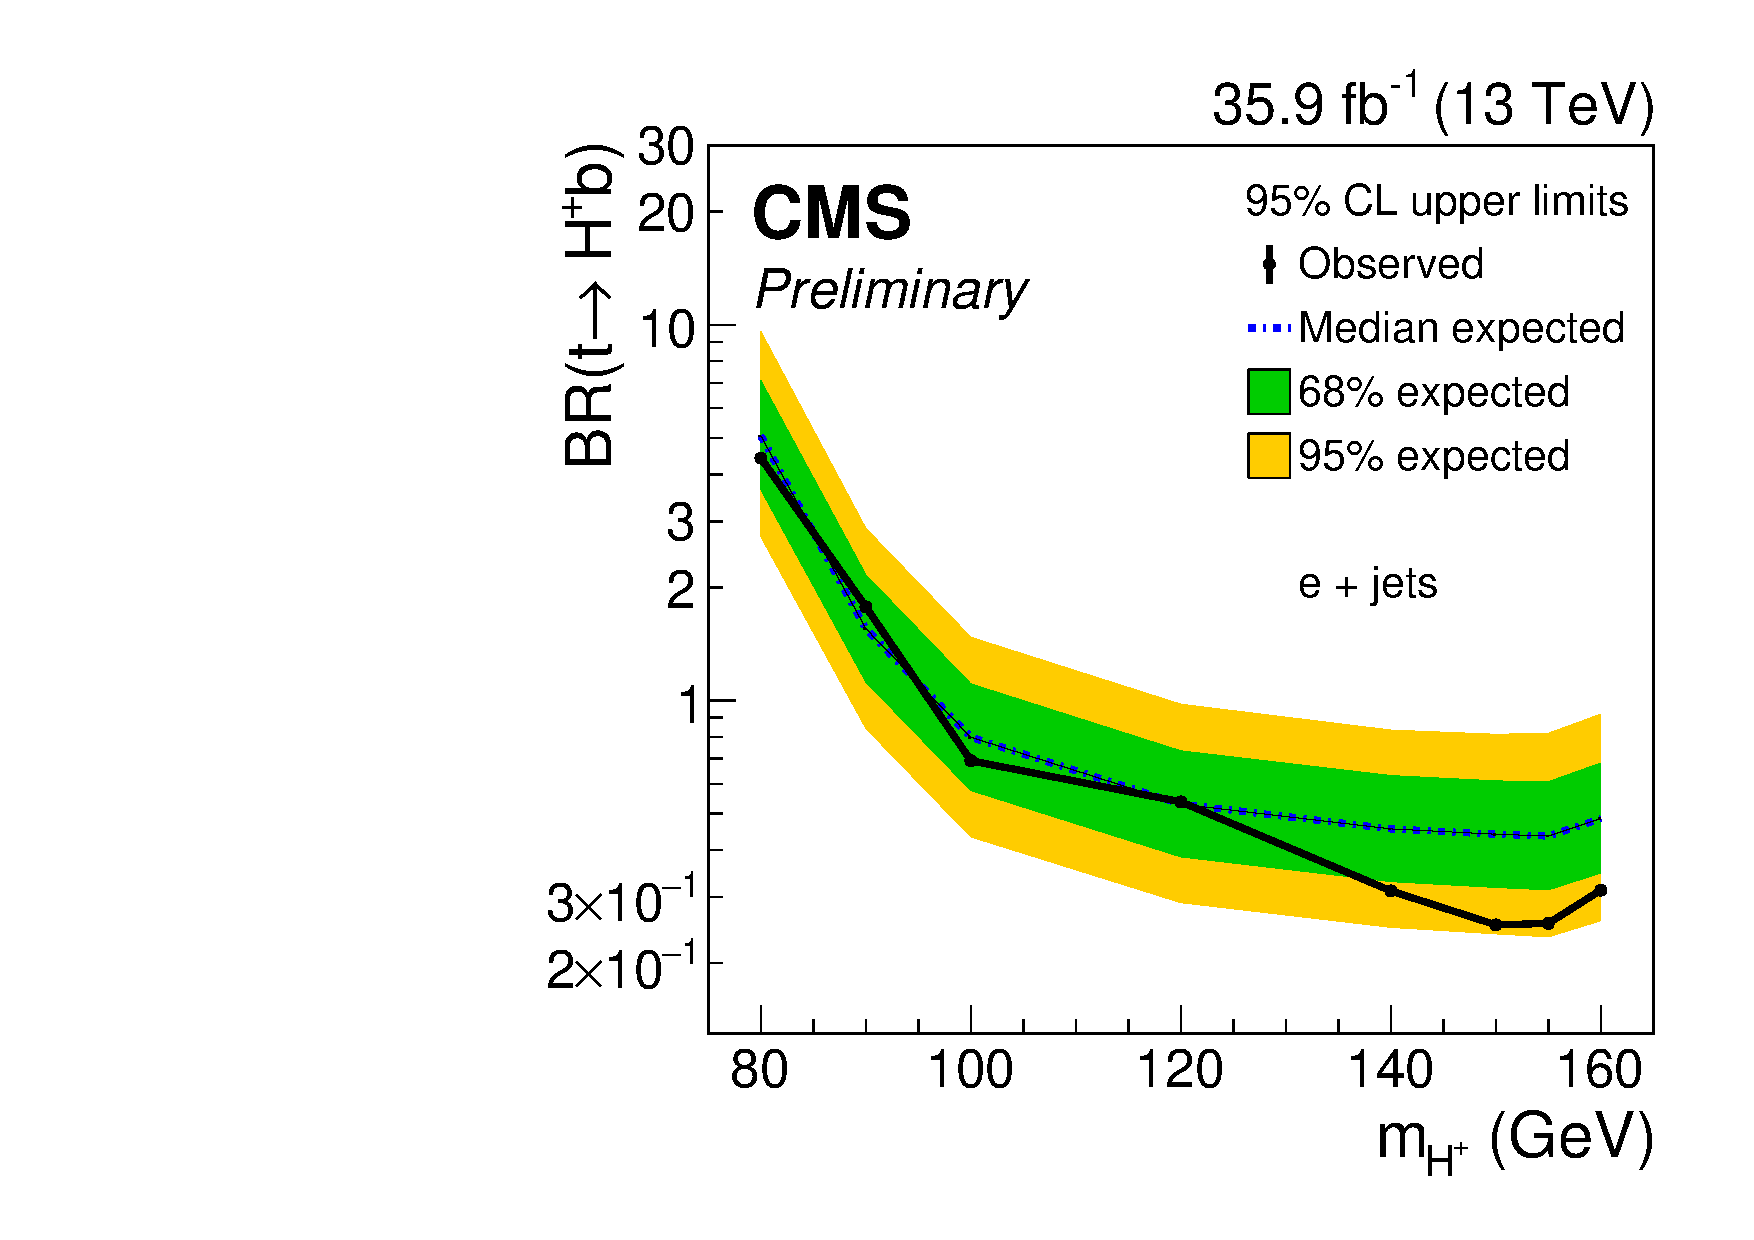
\includegraphics[width=0.30\linewidth]{Image/Limit/limit_pdf/limit_ele_Cat2_cTagInc.pdf}}
    \subfigure[With loose \PQc tagging \label{subfig:limit_lep_cTagL}]
    {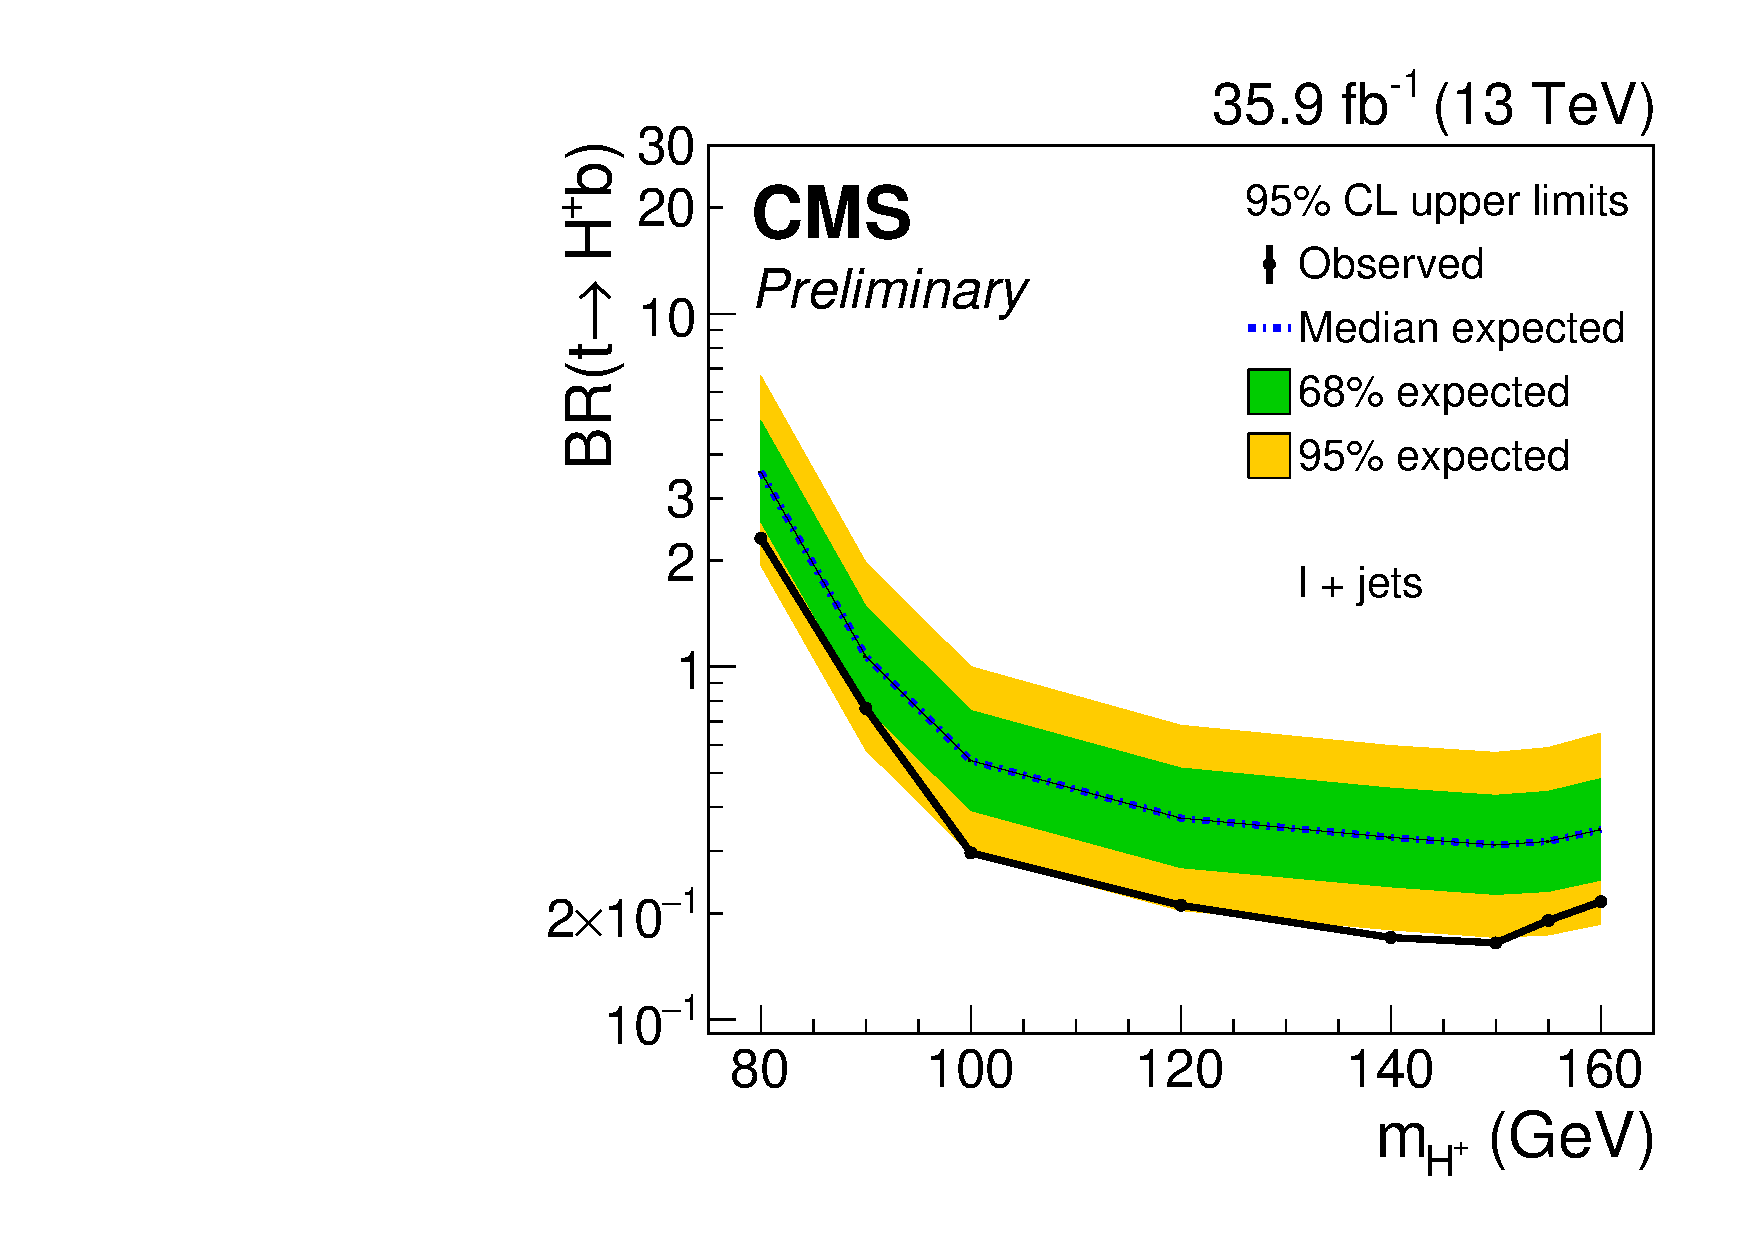
\includegraphics[width=0.30\linewidth]{Image/Limit/limit_pdf/limit_mu_ele_Cat2_cTagInc.pdf}}
\caption{The upper limit in \% on \brThb as a function of $m_{H^{+}}$ using $\mjj$ after kinematic fit
	selection without \PQc tagging, and with loose \PQc tagging, as discussed in 
	Section~\ref{ss:mjj_Inc} and \ref{ss:mjj_cTagL}, for \mujets, \ejets, and \ljets channel.}
    \label{fig:limit_cTagL}
\end{figure}


%-----------------------------------------
\section{Limits from inclusive event category with loose \text{c} tagging}
\label{ss:limit_cTagL}
%-----------------------------------------
The $\mjj$ distribution from the events with inclusive loose \PQc tagging as discussed 
in Section~\ref{ss:mjj_cTagL} are used to compute upper limits as shown in
Figures~\ref{subfig:limit_mu_cTagL}, \ref{subfig:limit_ele_cTagL}, and \ref{subfig:limit_lep_cTagL}. 
From these figures, it can be seen that the limits are marginally better compared to that 
of Figures~\ref{subfig:limit_mu_Inc}, ~\ref{subfig:limit_ele_Inc}, and \ref{subfig:limit_lep_Inc}. 
For different charged Higgs masses, the expected (observed) limits for loose \PQc tagging are in the 
range 0.40--1.41\% (0.26--0.82\%), 0.44--1.55\% (0.25--1.77\%), and 0.31--1.07\% (0.16--0.76\%)
for \mujets, \ejets, and \ljets channel, respectively.

%-----------------------------------------
\section{Limits from exclusive event categories based on \text{c} tagging}
\label{ss:limit_cTagEx}
%-----------------------------------------
\begin{figure}
    \centering  
    \subfigure[From combined exclusive charm categories.]
    {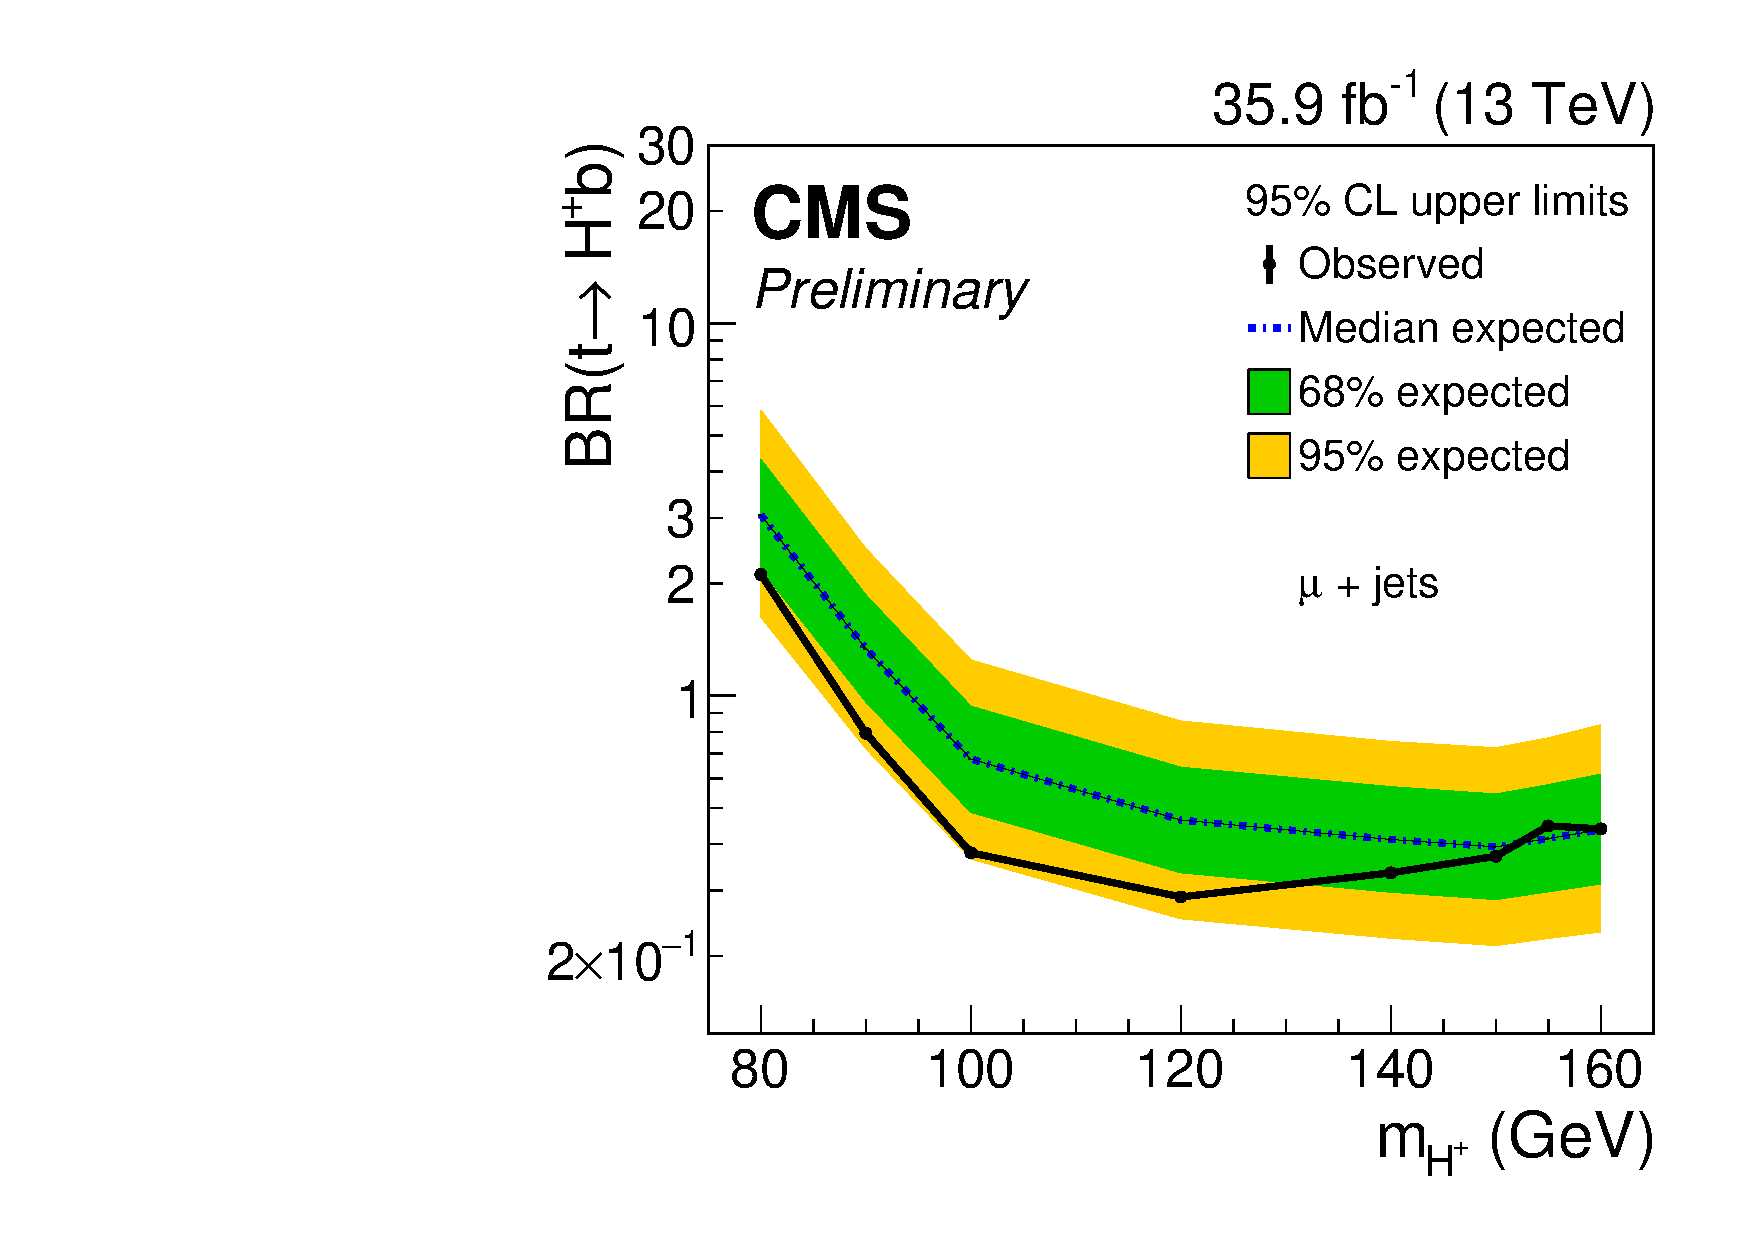
\includegraphics[width=0.45\linewidth]{Image/Limit/limit_pdf/limit_mu_Cat3_cTagEx.pdf}}
    \subfigure[From combined exclusive charm categories.]
    {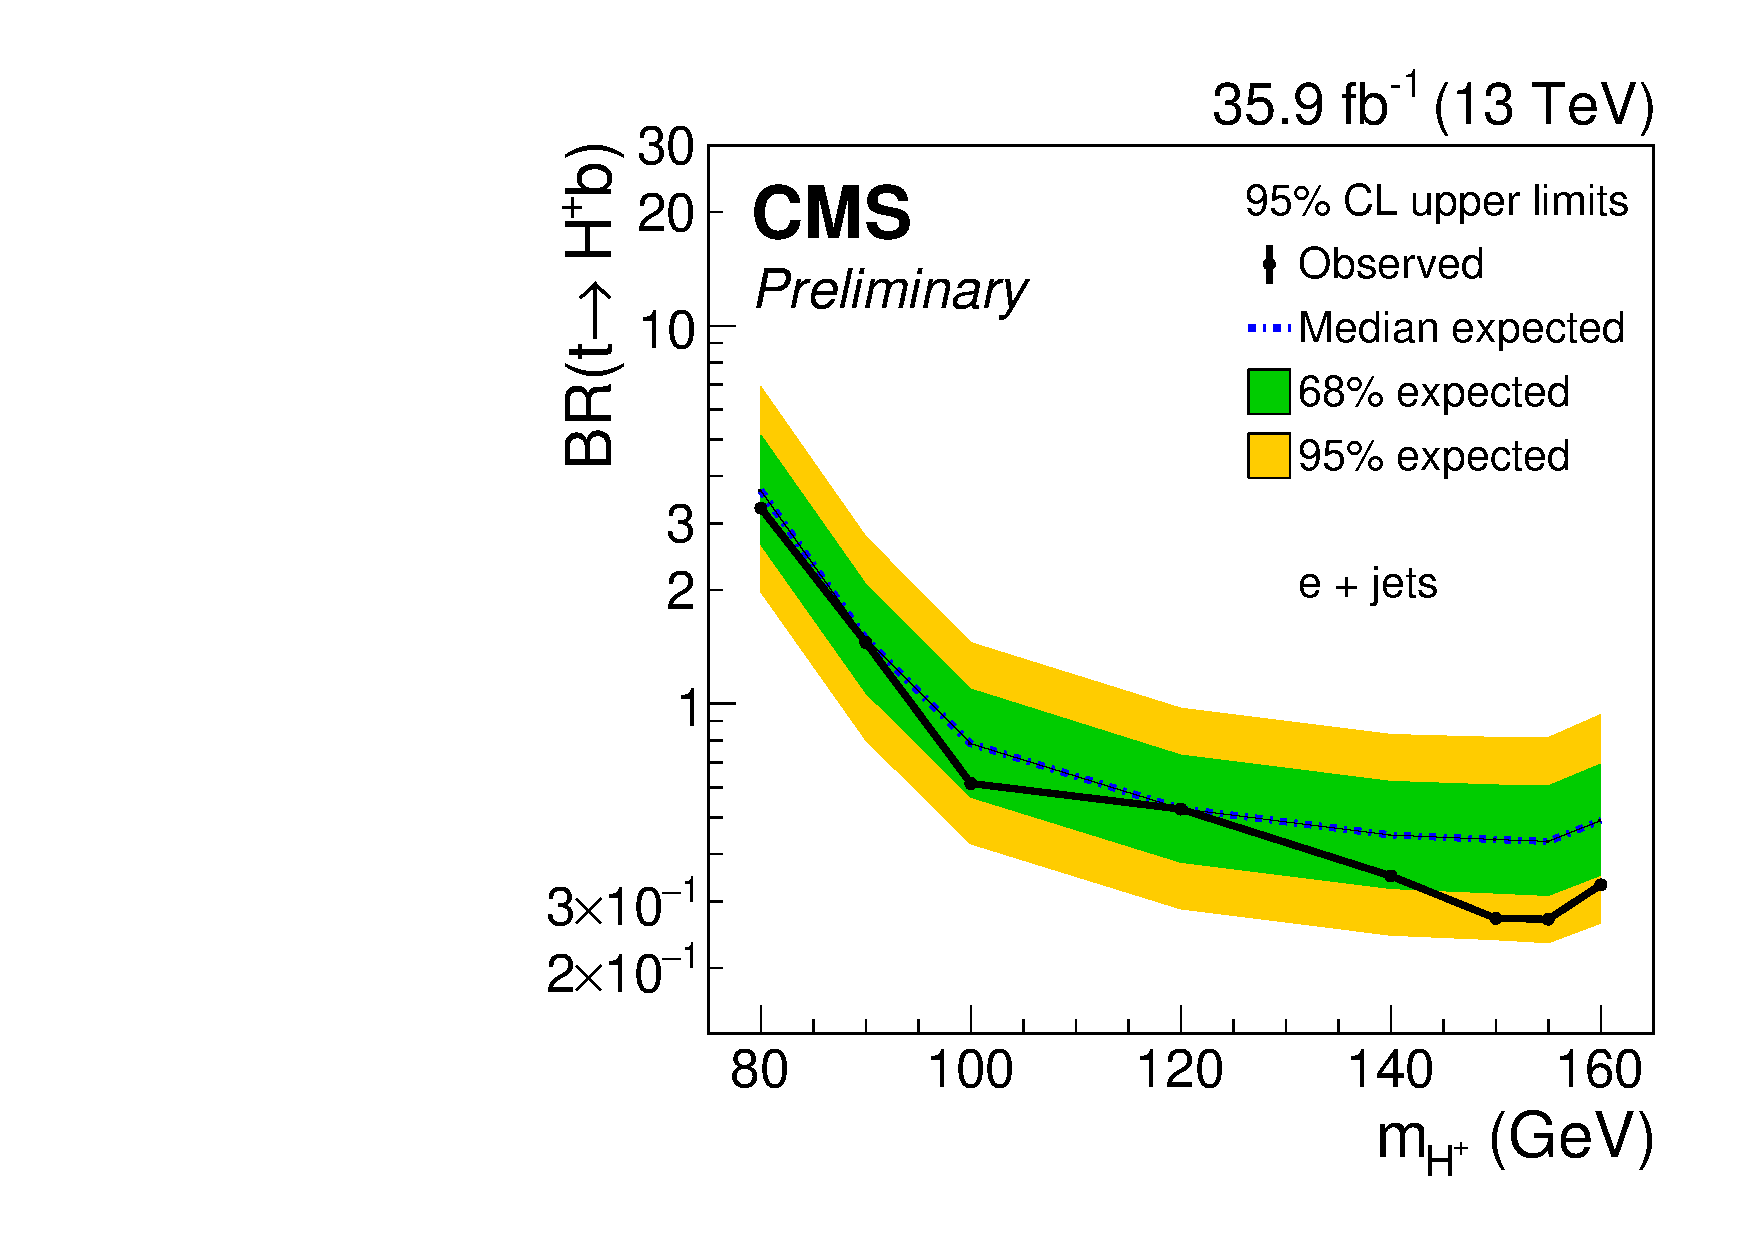
\includegraphics[width=0.45\linewidth]{Image/Limit/limit_pdf/limit_ele_Cat3_cTagEx.pdf}}
    \vfil
    \subfigure[From combined exclusive charm categories.]
    {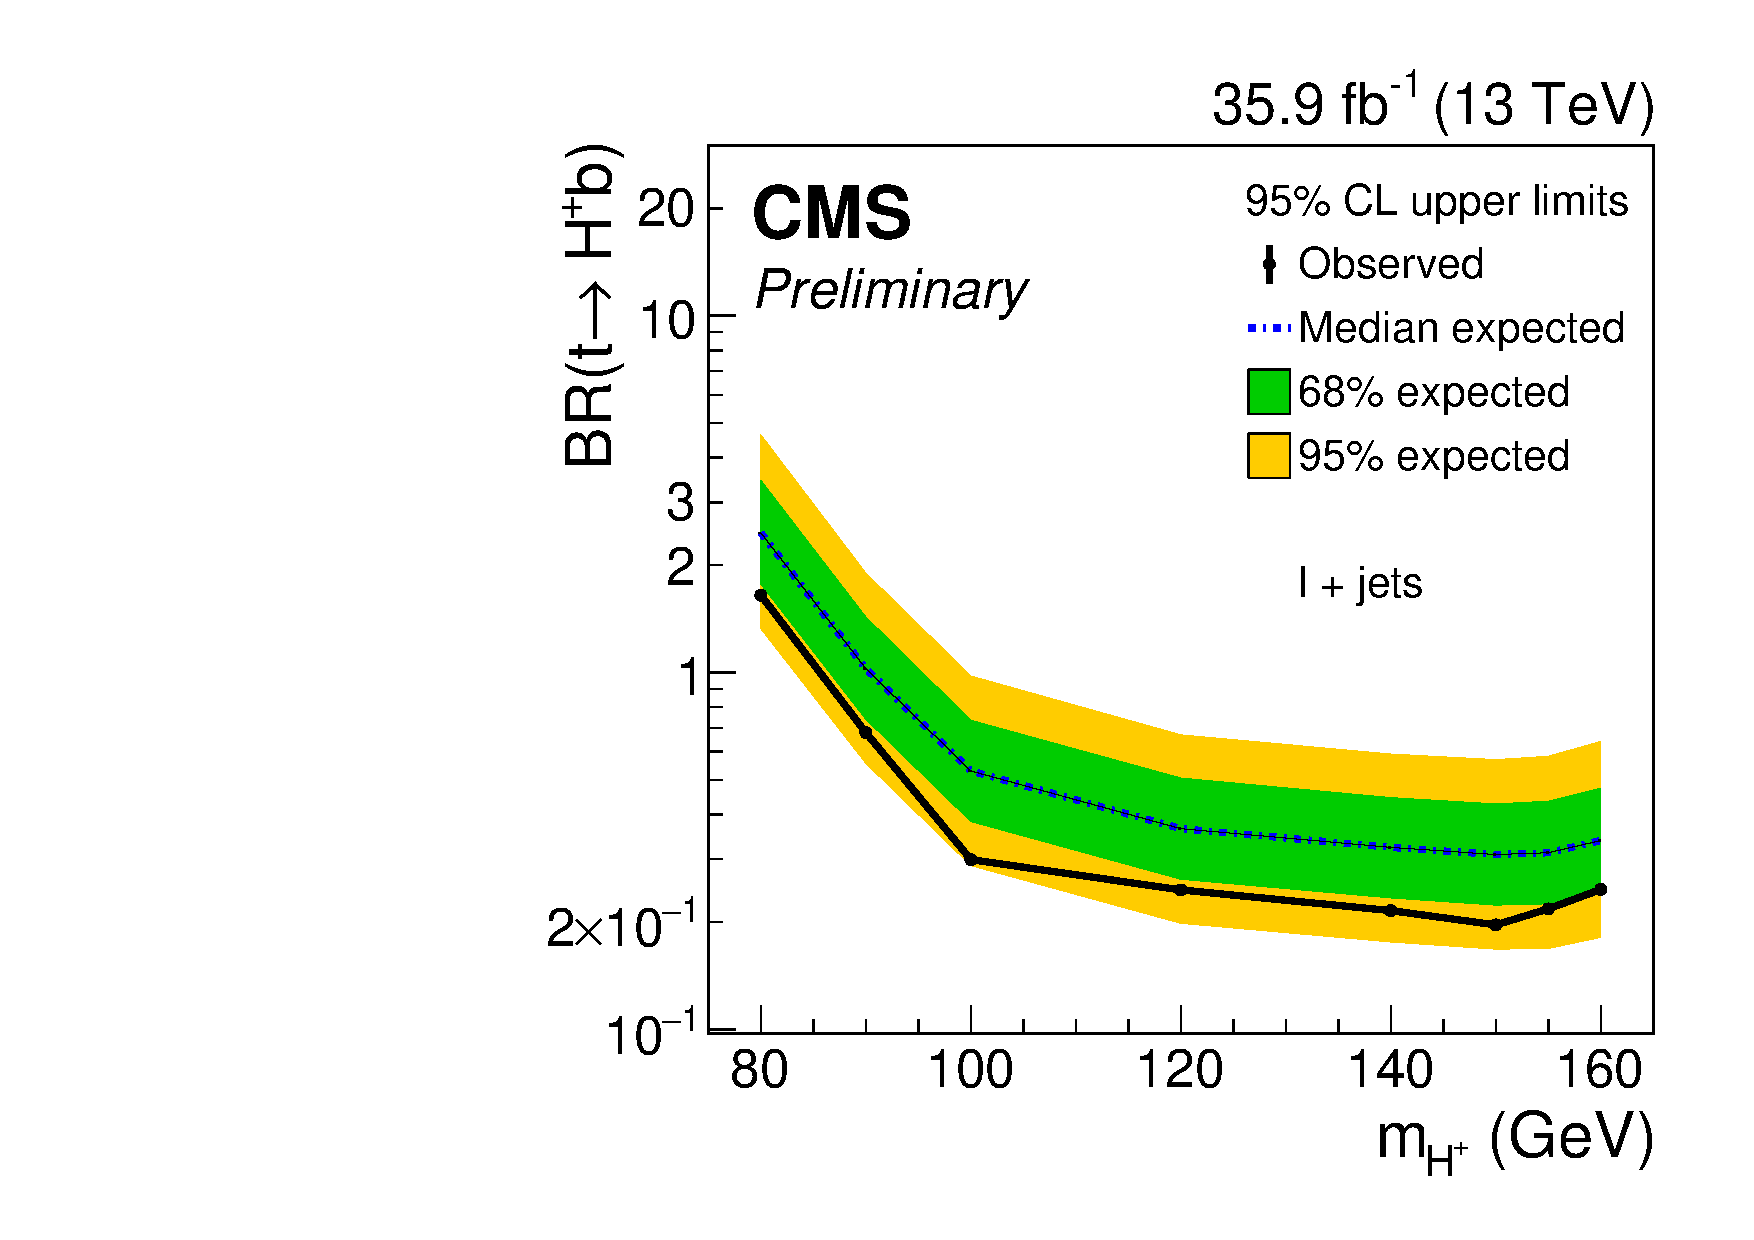
\includegraphics[width=0.60\linewidth]{Image/Limit/limit_pdf/limit_mu_ele_Cat3_cTagEx.pdf}}
	\caption{The upper limit in \% on \brThb as a function of $m_{H^{+}}$ by combining \mjj 
	distributions from different exclusive charm categories as discussed in 
	Section~\ref{ss:mjj_cTagEx} for \mujets \ejets, and \ljets channel.}
    \label{fig:limit_cTagEx}
\end{figure}

The signal significance is different in different charm categories as described in 
Section~\ref{ss:mjj_cTagEx}. The $\mjj$ distributions from loose, medium, and tight 
exclusive charm tagging categories are combined to compute the expected limits as shown in 
Figure~\ref{fig:limit_cTagEx}. From this figure, it can be seen that the upper limits
from exclusive categories are better compared to that obtained from inclusive working points.
For different charged Higgs masses, the expected (observed) limits from combined categories are 
in the range 0.39--1.34\% (0.29--0.79\%), 0.43--1.48\% (0.27--1.45\%), and 0.31--1.03\% (0.19--0.68)
for \mujets, \ejets, and \ljets channel, respectively.

\begin{figure}
    \centering  
    \subfigure[Expected limits.]
    {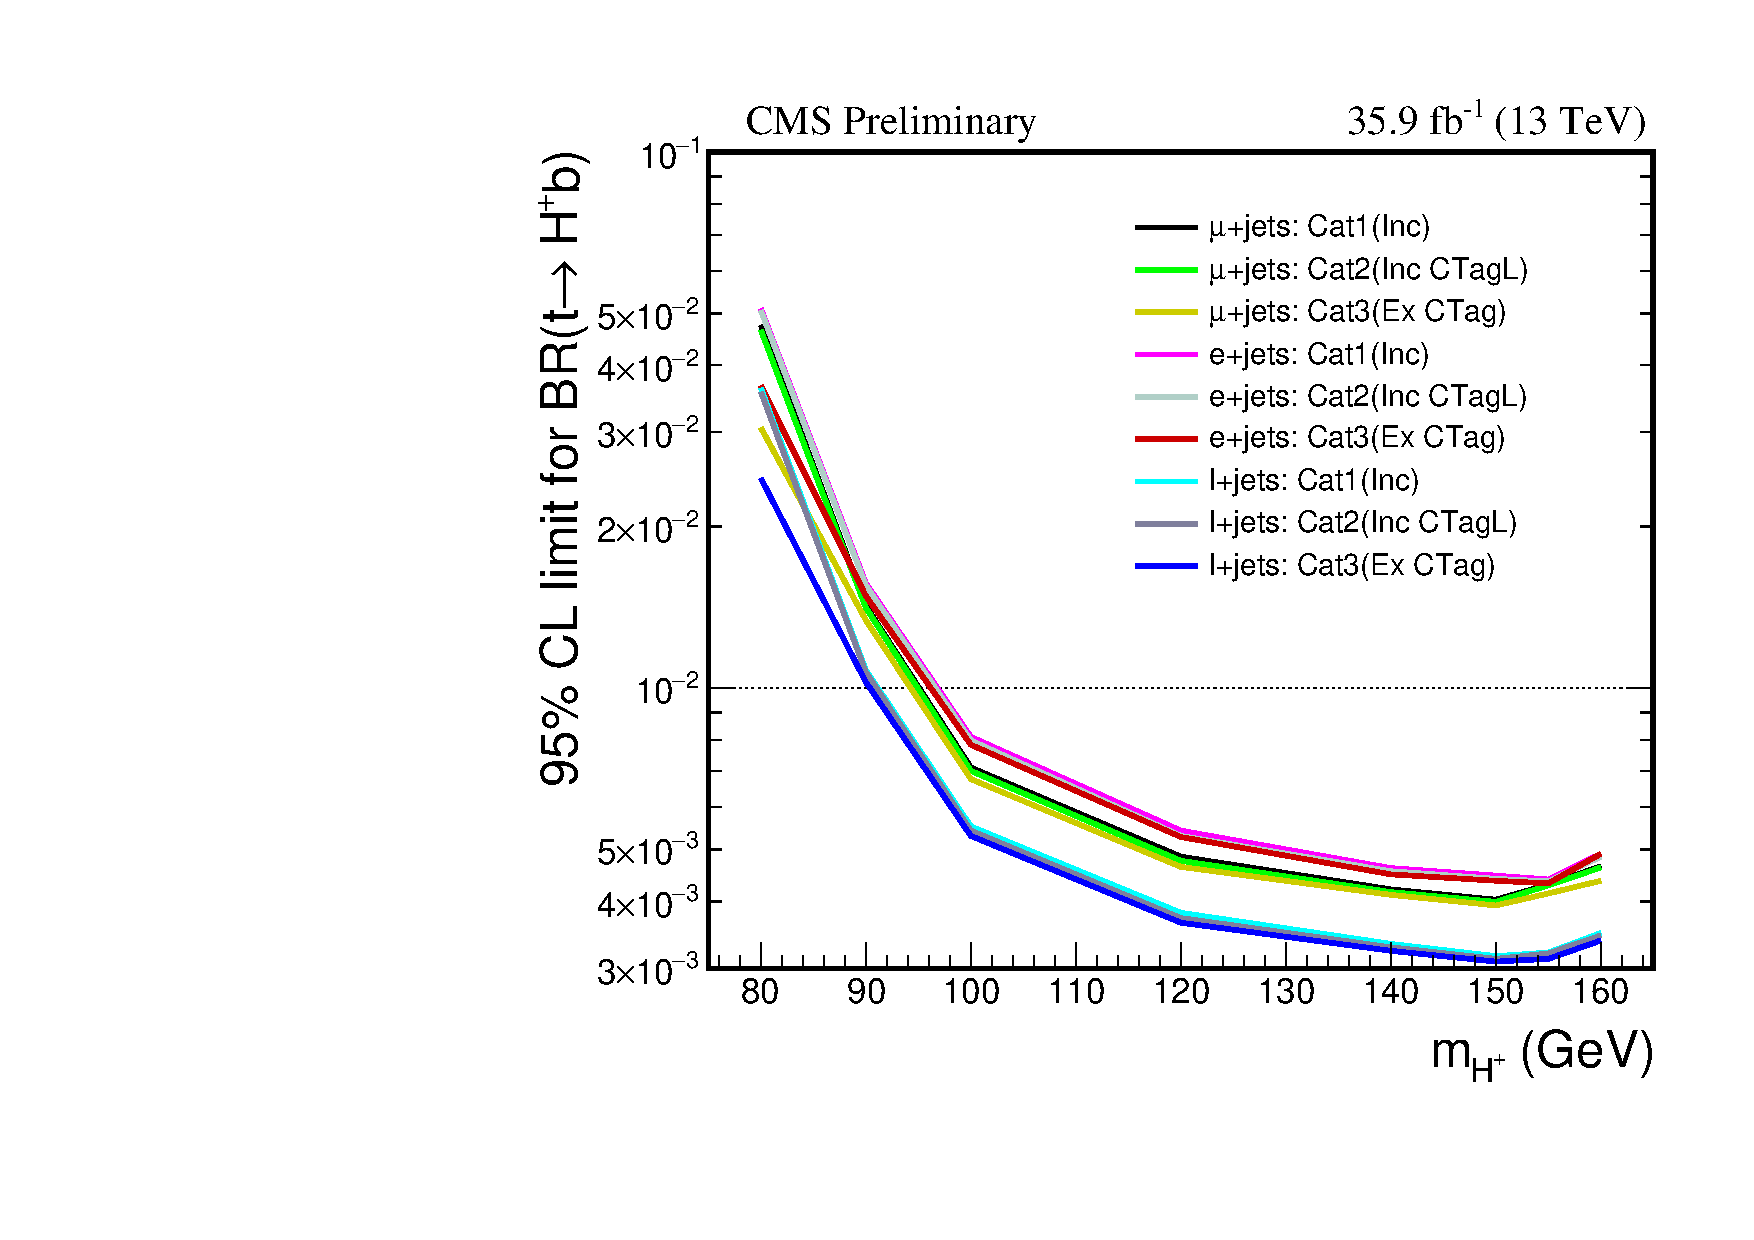
\includegraphics[width=0.6\linewidth]{Image/Limit/all_limits_expected.pdf}}
    \vfil
    \subfigure[Observed limits.]
    {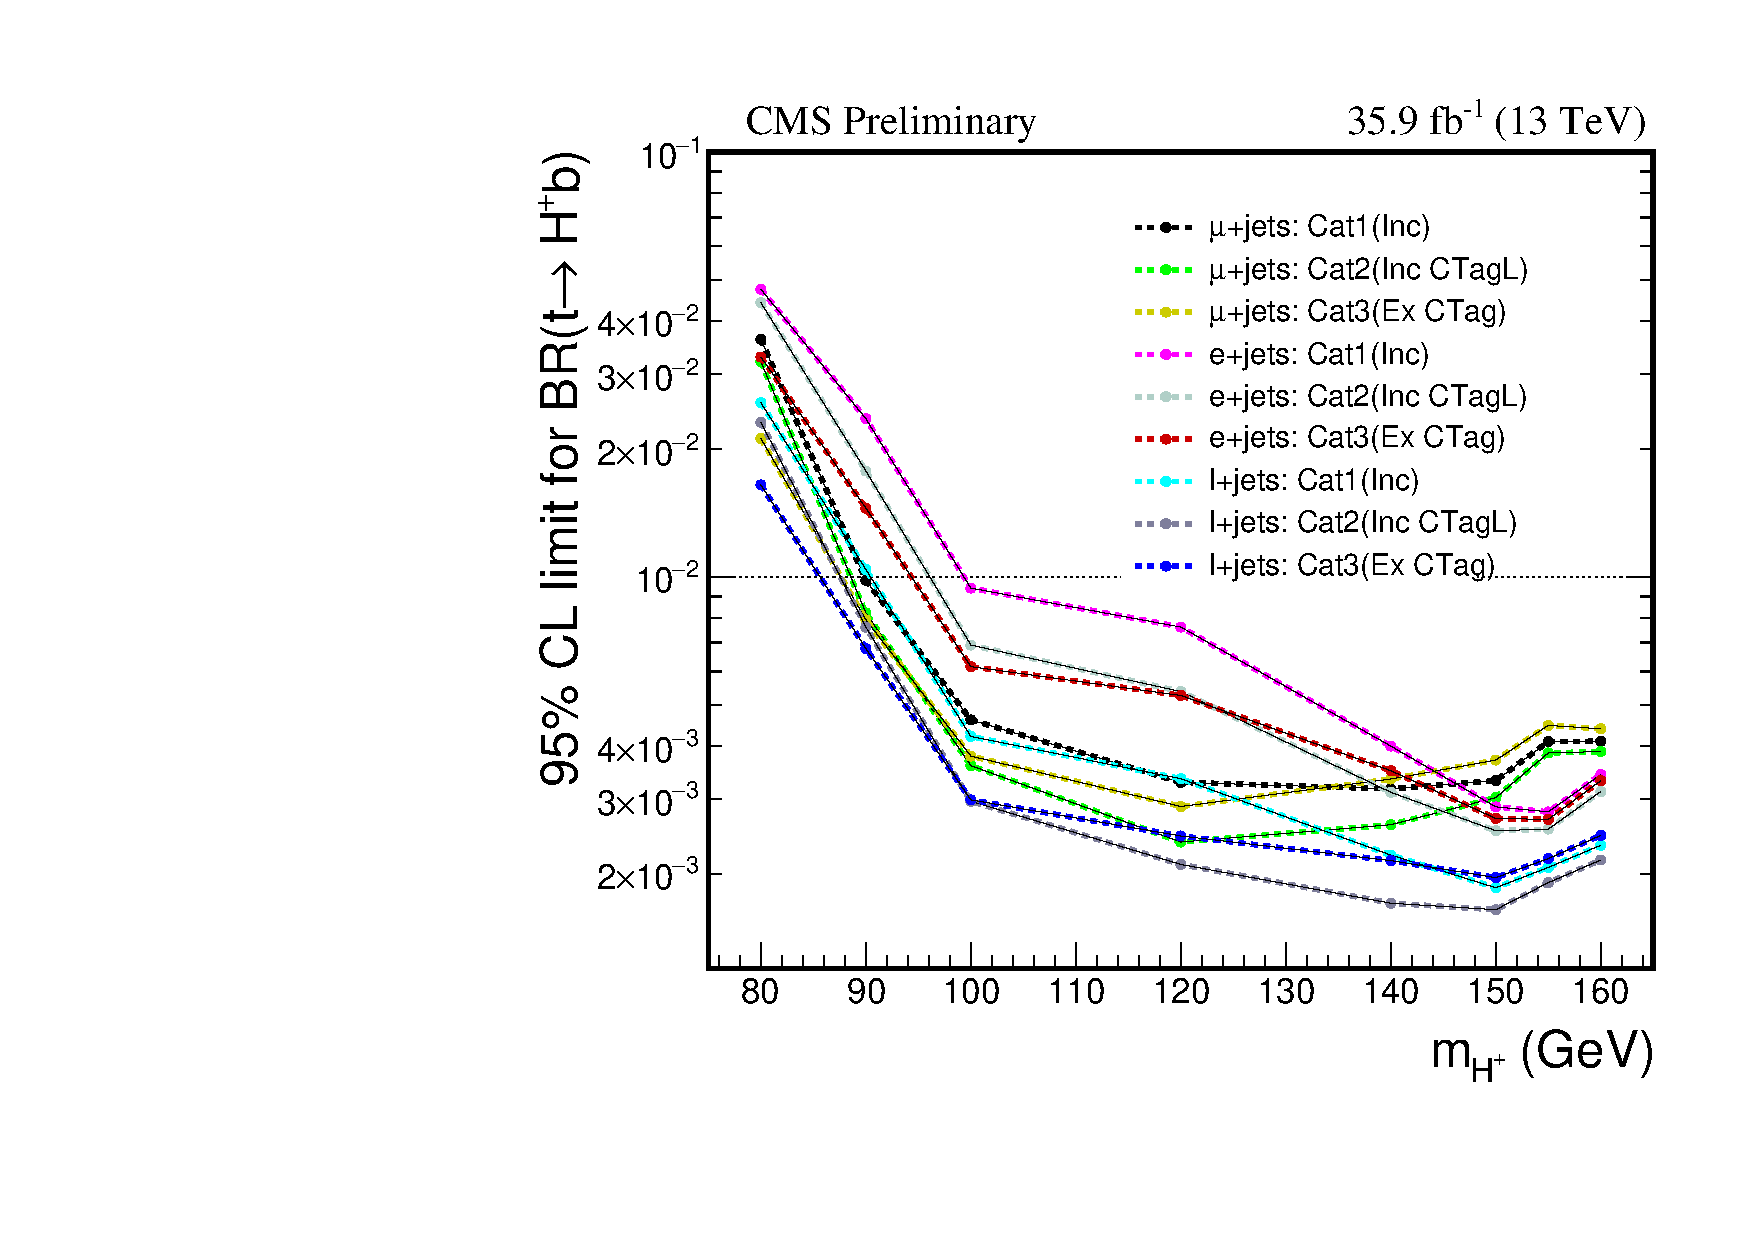
\includegraphics[width=0.6\linewidth]{Image/Limit/all_limits_observed.pdf}}
    \caption{The upper limit in \% on \brThb as a function of $m_{H^{+}}$ using $\mjj$ from 
	all event categories for \mujets, \ejets, and \ljets channel.}
\label{fig:finalLimit}
\end{figure}

\begin{table}
\caption{95\% CL exclusion limit in \% for \mujets channel from different event categories.}
\label{tab:limitMu}
\begin{center}
\begin{tabular}{ ccccccc}
\hline 
\hline 
\multicolumn{1}{c}{} & \multicolumn{2}{c}{$\mjj(Inc)$} & \multicolumn{2}{c}{$\mjj(Inc ~CTagL)$} & \multicolumn{2}{c}{$\mjj(Ex ~CTag)$} \\
  
{\bf{$\mHp$}} & Expected & Observed & Expected & Observed & Expected & Observed  \\ 
  
  (\GeV) & (\%) & (\%) & (\%) & (\%) & (\%) & (\%)  \\ 
 \hline 
\hline 
80  & $4.75^{+1.91}_{-1.33}$&3.62
 & $4.65^{+1.87}_{-1.32}$&3.21
 & $3.06^{+1.25}_{-0.873}$&2.12
\\
  
90  & $1.42^{+0.549}_{-0.399}$&0.982
 & $1.41^{+0.546}_{-0.396}$&0.823
 & $1.34^{+0.528}_{-0.376}$&0.793
\\
  
100  & $0.71^{+0.275}_{-0.198}$&0.461
 & $0.701^{+0.271}_{-0.195}$&0.36
 & $0.676^{+0.261}_{-0.19}$&0.379
\\
  
120  & $0.485^{+0.187}_{-0.134}$&0.329
 & $0.476^{+0.184}_{-0.131}$&0.238
 & $0.464^{+0.179}_{-0.129}$&0.288
\\
  
140  & $0.421^{+0.163}_{-0.116}$&0.317
 & $0.416^{+0.161}_{-0.115}$&0.261
 & $0.411^{+0.159}_{-0.115}$&0.335
\\
  
150  & $0.403^{+0.156}_{-0.111}$&0.332
 & $0.399^{+0.154}_{-0.111}$&0.303
 & $0.393^{+0.152}_{-0.109}$&0.371
\\
  
155  & $0.43^{+0.168}_{-0.12}$&0.41
 & $0.428^{+0.167}_{-0.119}$&0.385
 & $0.414^{+0.163}_{-0.116}$&0.447
\\
  
160  & $0.465^{+0.185}_{-0.131}$&0.411
 & $0.463^{+0.186}_{-0.13}$&0.388
 & $0.437^{+0.179}_{-0.125}$&0.439
\\
  
\hline 
\end{tabular}
\end{center}
\end{table}

\begin{table}
\caption{95\% CL exclusion limit in \% for \ejets channel from different event categories.}
\label{tab:limitEle}
\begin{center}
\begin{tabular}{ ccccccc}
\hline 
\hline 
\multicolumn{1}{c}{} & \multicolumn{2}{c}{$\mjj(Inc)$} & \multicolumn{2}{c}{$\mjj(Inc ~CTagL)$} & \multicolumn{2}{c}{$\mjj(Ex ~CTag)$} \\
  
{\bf{$\mHp$}} & Expected & Observed & Expected & Observed & Expected & Observed  \\ 
  
  (\GeV) & (\%) & (\%) & (\%) & (\%) & (\%) & (\%)  \\ 
 \hline 
\hline 
80  & $5.1^{+2.05}_{-1.43}$&4.75
 & $5.06^{+2.04}_{-1.42}$&4.42
 & $3.66^{+1.47}_{-1.03}$&3.29
\\
  
90  & $1.57^{+0.606}_{-0.437}$&2.35
 & $1.55^{+0.607}_{-0.432}$&1.77
 & $1.48^{+0.586}_{-0.417}$&1.45
\\
  
100  & $0.811^{+0.313}_{-0.226}$&0.941
 & $0.798^{+0.309}_{-0.222}$&0.691
 & $0.784^{+0.309}_{-0.218}$&0.615
\\
  
120  & $0.542^{+0.21}_{-0.15}$&0.762
 & $0.53^{+0.205}_{-0.146}$&0.537
 & $0.527^{+0.204}_{-0.147}$&0.526
\\
  
140  & $0.461^{+0.177}_{-0.127}$&0.4
 & $0.455^{+0.176}_{-0.126}$&0.311
 & $0.449^{+0.174}_{-0.125}$&0.35
\\
  
150  & $0.447^{+0.173}_{-0.124}$&0.288
 & $0.441^{+0.17}_{-0.123}$&0.253
 & $0.437^{+0.172}_{-0.122}$&0.27
\\
  
155  & $0.439^{+0.173}_{-0.123}$&0.28
 & $0.436^{+0.172}_{-0.122}$&0.255
 & $0.432^{+0.174}_{-0.121}$&0.269
\\
  
160  & $0.491^{+0.201}_{-0.138}$&0.343
 & $0.485^{+0.197}_{-0.137}$&0.313
 & $0.491^{+0.201}_{-0.139}$&0.332
\\
  
\hline 
\end{tabular}
\end{center}
\end{table}

\begin{table}
\caption{95\% CL exclusion limit in \% for \ljets channel from different event categories.}
\label{tab:limitLep}
\begin{center}
\begin{tabular}{ ccccccc}
\hline 
\hline 
\multicolumn{1}{c}{} & \multicolumn{2}{c}{$\mjj(Inc)$} & \multicolumn{2}{c}{$\mjj(Inc ~CTagL)$} & \multicolumn{2}{c}{$\mjj(Ex ~CTag)$} \\
  
{\bf{$\mHp$}} & Expected & Observed & Expected & Observed & Expected & Observed  \\ 
  
  (\GeV) & (\%) & (\%) & (\%) & (\%) & (\%) & (\%)  \\ 
 \hline 
\hline 
80  & $3.62^{+1.43}_{-1.02}$&2.57
 & $3.56^{+1.41}_{-0.993}$&2.31
 & $2.46^{+0.991}_{-0.691}$&1.65
\\
  
90  & $1.08^{+0.426}_{-0.298}$&1.04
 & $1.07^{+0.413}_{-0.298}$&0.762
 & $1.03^{+0.405}_{-0.286}$&0.678
\\
  
100  & $0.552^{+0.213}_{-0.154}$&0.421
 & $0.542^{+0.21}_{-0.151}$&0.297
 & $0.53^{+0.205}_{-0.148}$&0.299
\\
  
120  & $0.381^{+0.146}_{-0.105}$&0.335
 & $0.372^{+0.144}_{-0.103}$&0.211
 & $0.365^{+0.141}_{-0.102}$&0.246
\\
  
140  & $0.333^{+0.126}_{-0.0908}$&0.222
 & $0.328^{+0.124}_{-0.0907}$&0.171
 & $0.323^{+0.122}_{-0.0901}$&0.215
\\
  
150  & $0.316^{+0.122}_{-0.0873}$&0.186
 & $0.312^{+0.12}_{-0.0863}$&0.165
 & $0.309^{+0.119}_{-0.086}$&0.196
\\
  
155  & $0.321^{+0.127}_{-0.0883}$&0.207
 & $0.32^{+0.124}_{-0.0891}$&0.191
 & $0.312^{+0.123}_{-0.0878}$&0.218
\\
  
160  & $0.349^{+0.139}_{-0.0981}$&0.234
 & $0.345^{+0.136}_{-0.097}$&0.216
 & $0.338^{+0.136}_{-0.0958}$&0.247
\\
  
\hline 
\end{tabular}
\end{center}
\end{table}

